\documentclass[12pt]{article}
\usepackage[utf8]{inputenc}
\usepackage[T1]{fontenc} % uses T1 fonts (better quality)
\usepackage{lmodern}
\usepackage[dvipsnames]{xcolor}
\usepackage[margin=2cm]{geometry}
\geometry{top=1.5cm}
\usepackage{graphicx} \graphicspath{ {./Images/} }
\usepackage{pdfpages}
\usepackage{booktabs}   % for table borders
\usepackage{amsmath,bm,amssymb}
\usepackage{mathtools}
\usepackage[makeroom]{cancel}
\usepackage{tikz} \usetikzlibrary{shapes,arrows}
% \usepackage{minted} \usemintedstyle{friendly}
\usepackage{enumitem}
\makeatletter
\renewcommand{\thefigure}{9.\@arabic\c@figure}
\definecolor{CrispBlue}{HTML}{0176AE}
\makeatother

\begin{document}
 	\begin{center}
    \line(1,0){300}\\[0.25cm]
 	\Large{\bfseries ECE540: Homework \#5}\\
 	\textsc{\large David Kirby}\\
 	\textsc{\large Due: 22 November 2020}\\
 	\line(1,0){300}\\[0.75cm]
 	\end{center}
\section*{Chapter 9 (\(\bm{7^{th}}\) Edition)}
\subsection*{Review Questions}
\begin{enumerate}
		\subsubsection*{Section 9.2}
	\item R6. List three disadvantages of UDP streaming.\par
		\color{CrispBlue}
		\begin{itemize}
			\item UDP doesn't transmit at constant rate or with continuous playout.
			\item A media control server is required, creating larger overhead and more complexity.
			\item Many firewalls do not allow UDP.
		\end{itemize}
		\color{black}
	\vspace{-2em}\subsubsection*{Section 9.3}
	\item R9. What is the difference between end-to-end delay and packet jitter? What are the causes of packet jitter?\par
		\color{CrispBlue}End-to-end delay is the amount of time it takes a packet to go from source to destination. It is the accumulation of transmission, processing, and queuing delays in routers; propagation delays in links; and end-system processing delays. Packet jitter is the fluctuation in end-to-end delays between packets. Congestion, low bandwidth links, and changing paths can all cause packet jitter.\color{black}
	\item R10. Why is a packet that is received after its scheduled playout time considered lost?\par
		\color{CrispBlue}Packets have a limited time window, if a packet arrives after this window (playout time), it will expire and be discarded. Since it is discarded, it will be considered lost.\color{black}
	\vspace{-1em}\subsubsection*{Section 9.4}
	\item R12. How are different RTP streams in different sessions identified by a receiver? How are different streams from within the same session identified?\par
	\color{CrispBlue}
		\begin{itemize}
			\item RTP streams have multicast addresses and provide one-to-many and many-to-many multicast trees.
			\item A Synchronization Source Identifier is sent with each stream that identifies streams within the same session.
		\end{itemize}
	\color{black}
\vspace{-1em}
\end{enumerate}\newpage
\subsection*{Problems}
\begin{enumerate}
	\item P2. Recall the simple model for HTTP streaming shown in Figure 9.3. Recall that \(B\) denotes the size of the client’s application buffer, and \(Q\) denotes the number of bits that must be buffered before the client application begins playout. Also \(r\) denotes the video consumption rate. Assume that the server sends bits at a constant rate \(x\) whenever the client buffer is not full.
	\setcounter{figure}{2}
	\begin{figure}[h!]
	\centering
	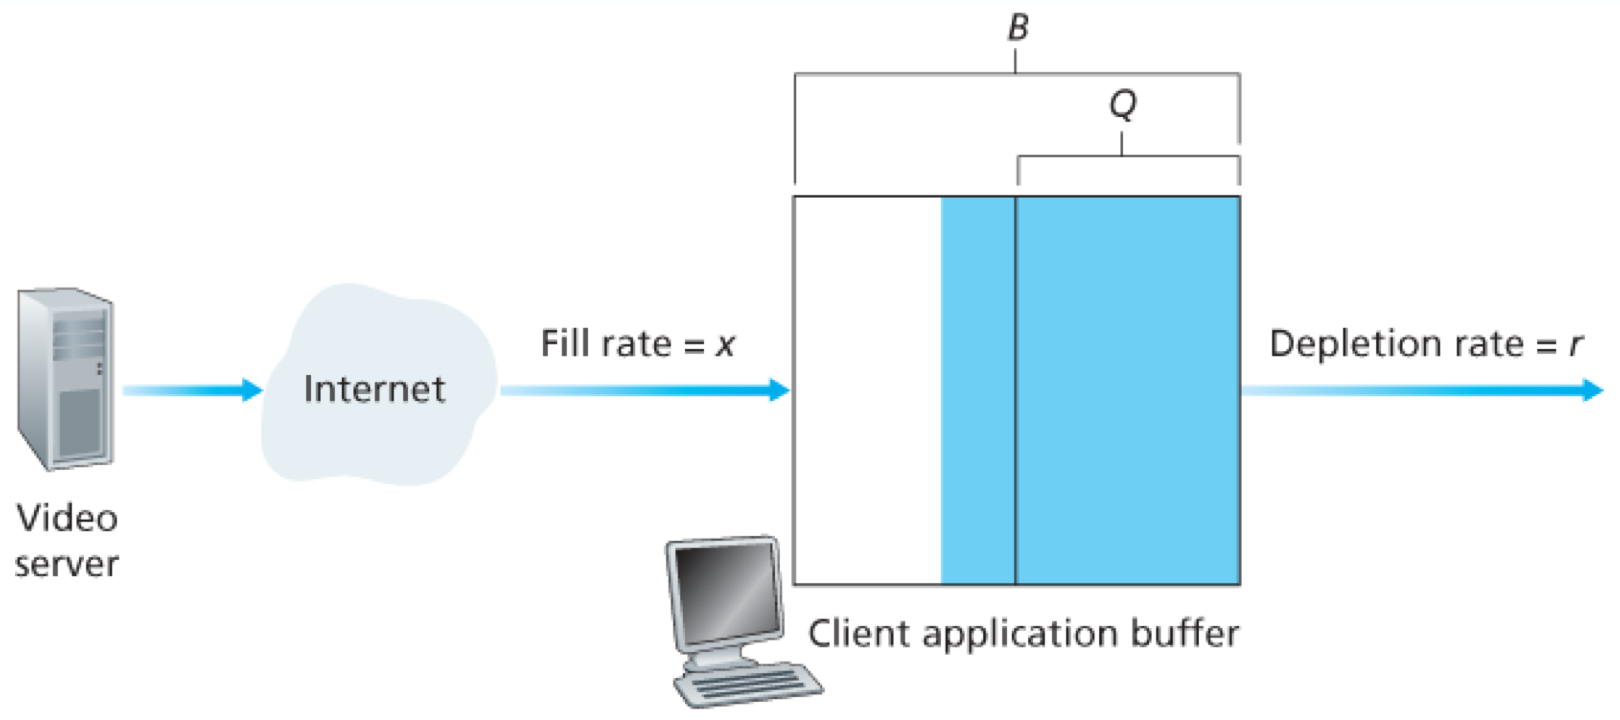
\includegraphics[width=0.6\textwidth]{./Images/Fig09-003.png}
	\caption{Analysis of client-side buffering for video streaming}
	\end{figure}
		\begin{enumerate}
			\item Suppose that \(x<r\). As discussed in the text, in this case playout will alternate between periods of continuous playout and periods of freezing. Determine the length of each continuous playout and freezing period as a function of \(Q, r, \) and \(x\).\\[1em]
			\color{CrispBlue}
			Since the server cannot send bits as quickly as the video is consuming them, the continuous playout and freezing period will be bottle-necked at \(\displaystyle\frac{Q}{x}\)\color{black}
			\item Now suppose that \(x>r\). At what time \(t=t_f\) does the client application buffer become full?\\[1em]
			\color{CrispBlue}
			Since the server is sending bits quicker than the video can consume, the buffer will fill up. This will happen at a rate of \(\displaystyle\frac{Q}{x}+\displaystyle\frac{B-Q}{x-r}\)\color{black}
		\end{enumerate}
	\item P6. In the VoIP example in Section 9.3, let \(h\) be the total number of header bytes added to each chunk, including UDP and IP header.\par
		\begin{enumerate}
			\item Assuming an IP datagram is emitted every 20 msecs, find the transmission rate in bits per second for the datagrams generated by one side of this application.
			\color{CrispBlue}
			\begin{align*}
				\text{datagram} = 160\text{ bytes}+h&&\# \text{ datagrams}= \frac{1}{20\text{ msecs}}=50
			\end{align*}
			\begin{align*}
				r_{\text{trans}}&=50 \cdot 8\text{ bits}\cdot (160\text{ bytes}+h)\\
				&=64+0.4h \text{ kbps}
			\end{align*}
			\color{black}
			\item What is a typical value of \(h\) when RTP is used?\\[1em]
			\color{CrispBlue}
			The typical value is the UDP header + IP header + RTP header, so 40 bytes.
			\color{black}
		\end{enumerate}
	\item P10. Compare the procedure described in Section 9.3 for estimating average delay with the procedure in Section 3.5 for estimating round-trip time. What do the procedures have in common? How are they different?\par
	\color{CrispBlue}
	Estimating average delay and estimating round-trip time both use the same formula and both use previously calculated delays. RTT calculates the entire trip time, while average delay only calculates source to destination (not including queueing delays). For RTT, each segment is count, for estimating average delay, only counted once it has been received.
	\color{black}
	\item P15.
		\begin{enumerate}
			\item Suppose we send into the Internet two IP datagrams, each carrying a different UDP segment. The first datagram has source IP address \(A_1\), destination IP address \(B\), source port \(P_1\), and destination port \(T\). The second datagram has source IP address \(A_2\), destination IP address \(B\), source port \(P_2\), and destination port \(T\). Suppose that \(A_1\) is different from \(A_2\) and that \(P_1\) is different from \(P_2\). Assuming that both datagrams reach their final destination, will the two UDP datagrams be received by the same socket? Why or why not?\par
			\color{CrispBlue}
			Yes, both UDP datagrams will be received by the same socket since both have the same destination IP and port. The receiver has a demultiplexer to resolve these.
			\color{black}
			\item Suppose Alice, Bob, and Claire want to have an audio conference call using SIP and RTP. For Alice to send and receive RTP packets to and from Bob and Claire, is only one UDP socket sufficient (in addition to the socket needed for the SIP messages)? If yes, then how does Alice’s SIP client distinguish between the RTP packets received from Bob and Claire?\par
			\color{CrispBlue}
			Yes, one UDP socket is sufficient. Each of Bob and Alice's RTP packets will have their own IP addresses.
			\color{black}
		\end{enumerate}
	\item P20. Consider the leaky bucket policer that polices the average rate and burst size of a packet flow. We now want to police the peak rate, \(p\), as well. Show how the output of this leaky bucket policer can be fed into a second leaky bucket policer so that the two leaky buckets in series police the average rate, peak rate, and burst size. Be sure to give the bucket size and token generation rate for the second policer.\par
	\color{CrispBlue}
	Please see modified figure below. Bucket size = 1 token, token generation rate = \(p\ \frac{\text{tokens}}{\text{sec}}\).
	\begin{figure}[h!]
		\centering
		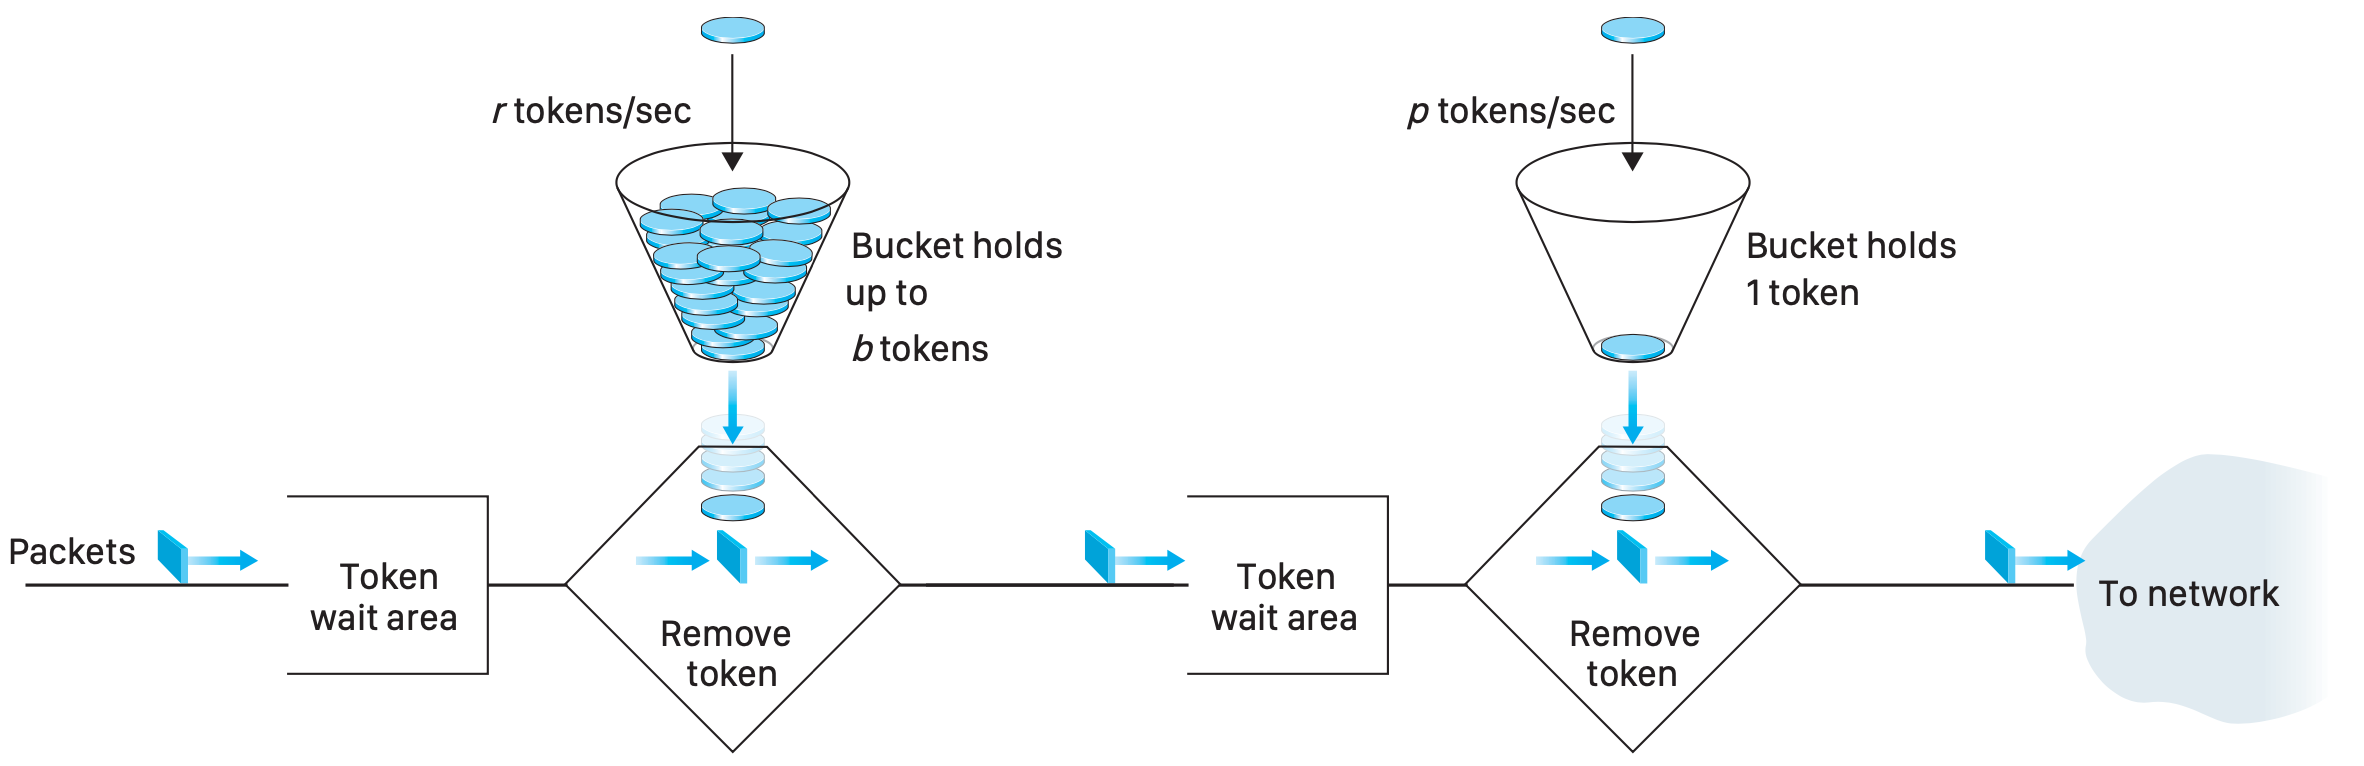
\includegraphics[width=0.9\textwidth]{./Images/Fig09-000.png}
		\end{figure}
	\color{black}
\end{enumerate}
\end{document}